The dataset format remains unchanged. The pairs of images are divided between 4 seasons and are grouped by regions into specific folders. However, the data acquiring process has been changed slightly. On top of using Google Earth Engine\cite{GORELICK201718} we also use the Copernicus Data Space Ecosystem API to access Sentinel data.

\subsection{Image format}
The images are in png format with the dimension of $256\times256$ pixels. The scale or zoom level of the image in terms of distance is 20m. Now, the sentinel satellite specific image details will be defined in the following points:
\begin{itemize}
    \item \textbf{Sentinel-1:} The images are taken from the IW acquisition mode of the satellite and are in VV polarization. It comprises of only a single band.
    \item \textbf{Sentinel-2:} The images consist of 3 bands for Red, Green and Blue. The bands are also scaled for proper visualisation.
\end{itemize}

\subsection{Copernicus API Method}
Copernicus Data Space Ecosystem with a tagline of Europe's eyes on Earth is an open ecosystem that provides free instant access to a wide range of data and services from the Copernicus Sentinel missions\cite{copernicusHome}. It provides data from all Sentinel satellites in various forms. For Sentinel-1 images, we used the 'Level 3 Monthly Mosaics' collection, and for Sentinel-2 we used the 'Level 3 Quaterly Mosaics' collection.
The following sections contain an overview of how the copernicus API was used to obtain the images.

\subsubsection{Generating coordinates}
The Copernicus service provides a limited number of API calls per month for free users (30,000 calls). To maximize efficiency of API call usage, we decided to obtain images of the maximum size limit offered by Copernicus. The maximum limit is $2500\times2500$ pixels per image. Now, the scale of images in SEN1-2 dataset is 20m.

\begin{align*}
    \text{Hence, ground distance per pixels} &= 20m \\
    \text{Total distance for 2500x image is} &= 20\times2500 \\
    &= 50,000m
\end{align*}

Thus, we need to create square patches with 50 KM distances as the side of the said patch. For this task, we first select a region in Google Earth Engine using the rectangular selection tool. We can then obtain the coordinates for the four corners of the selection. We use these coordinates to divide the region into multiple square regions with 50 KM side. To perform the division we calculate subsequent latitude and longitude coordinates beginning from the top left corner of the selection. The formula for approximately converting Longitude and Latitude into kilometers are:

\begin{itemize}
    \item \textbf{Latitude: } $1^\circ = 110.574$KM
    \item \textbf{Longitude:} $1^\circ = 111.320\times cos(latitude)$ KM
\end{itemize}

Thus, we end up with a list of coordinates for all subregions formed from the original selection.

\subsubsection{Authentication}
In order to use the API of copernicus sentinel hub, we need to authenticate ourselves and obtain an access token. Therefore, client id and client secret are used to fetch a token and authenticate ourself.

\subsubsection{Defining Image properties}
AFter authentication, the image properties are set in preparation of the image download. This is where the difference in obtaining Sentinel-1 and Sentinel-2 images appear due to differences in image formats.

We set the image height and width to 2500 pixels each. Following that, the eval script is set. An eval script is a piece of Javascript code which defines how the satellite data shall be processed by Sentinel Hub\cite{evalDoc}. Two different eval scripts are used for Sentinel-1 and Sentinel-2 images due to different number of bands being used in the images.

The Sentinel-1 eval script is as follows:

\begin{lstlisting}
    //VERSION=3
    function setup() {
        return {
            input: ["VV"],
            output: { bands: 1 }
        };
    }

    function evaluatePixel(sample) {
        return [sample.VV];
    }
\end{lstlisting}

The Sentinel-2 eval script is as follows:

\begin{lstlisting}
    //VERSION=3
    function setup() {
        return {
            input: ["B02", "B03", "B04"],
            output: { bands: 3 }
        };
    }

    function evaluatePixel(sample) {
        return [2.5 * sample.B04/10000, 2.5 * sample.B03/10000, 2.5 * sample.B02/10000];
    }
\end{lstlisting}

From the eval scripts we can infer that Sentinel-1 images have one band, called "VV". It is the polarization of the captured image. "VV" is vertical polarization, i.e.,  vertically transmit and vertically receive. And Sentinel-2 images have 3 bands, namely, B02, B03, B04. The bands are for Blue, Green, and Red channel respectively. The Sentinel-2 images are also preprocessed before download by scaling and normalizing the pixel values. 

Then, bounding box coordinates and time frame for images are sent with the request along with the previously mentioned data.

\subsubsection{Adding Region Data}
Now, the new addition in our dataset is the temperature region information. Temperature regions are also known as heat zones of the Earth. There are three heat zones, Arctic or Frigid zone, Temperate zone, and Tropical or Torrid Zone. These zones are classified according to latitude.

\begin{itemize}
    \item Tropical Zone: It lies between the Tropic of Cancer ($23.5^\circ$ North) and Tropic of Capricorn ($23.5^\circ$ South). This zone receives the most heat from the sun.
    \item Temperate Zone: In the northern hemisphere, this zone lies between Tropic of Cancer and the Arctic circle ($66.5^\circ$ North). In the southern hemisphere, it lies between Tropic of Capricorn and Antarctic circle ($66.5^\circ$ South).This region is moderately cooler compared to the tropical region.
    \item Arctic Zone: In the northern hemisphere, it is located between the North Pole ($90^\circ$ North) and Arctic circle. In the southern hemisphere, it lies between the South Pole ($90^\circ$ South) and the Antarctic circle. This region is the coldest region of them all.
\end{itemize}

We have decided to include lesser amounts of arctic zone data as those images majorly consist of snow wihtout much variation.

Therefore, the region is calculated based on the latitude and is written to a csv file. The csv files are made on a per region folder basis.

\subsubsection{First manual inspection}
Once the images are downloaded, the first manual inspection is performed. We check the pair of images to verify that the images contain visible patterns and variations throughout its entirety. Images which had regions of no variation were discarded.

Moreover, unlike the original dataset, cloud coverage was not an issue as the Sentinel-2 Monthly Mosaics were cloud optimized images.

\subsubsection{Cropping images}
After the first manual inspection, the images were cropped and divided into multiple smaller images to match the dimensions of the original dataset. The downloaded images have a dimension of $2500\times2500$ pixels. They are divided into 81 $256\times256$ sized images each. This results in a minor loss of information. Figure \ref{fig:cropStep} shows the visualisation of this step.

\begin{figure*}
    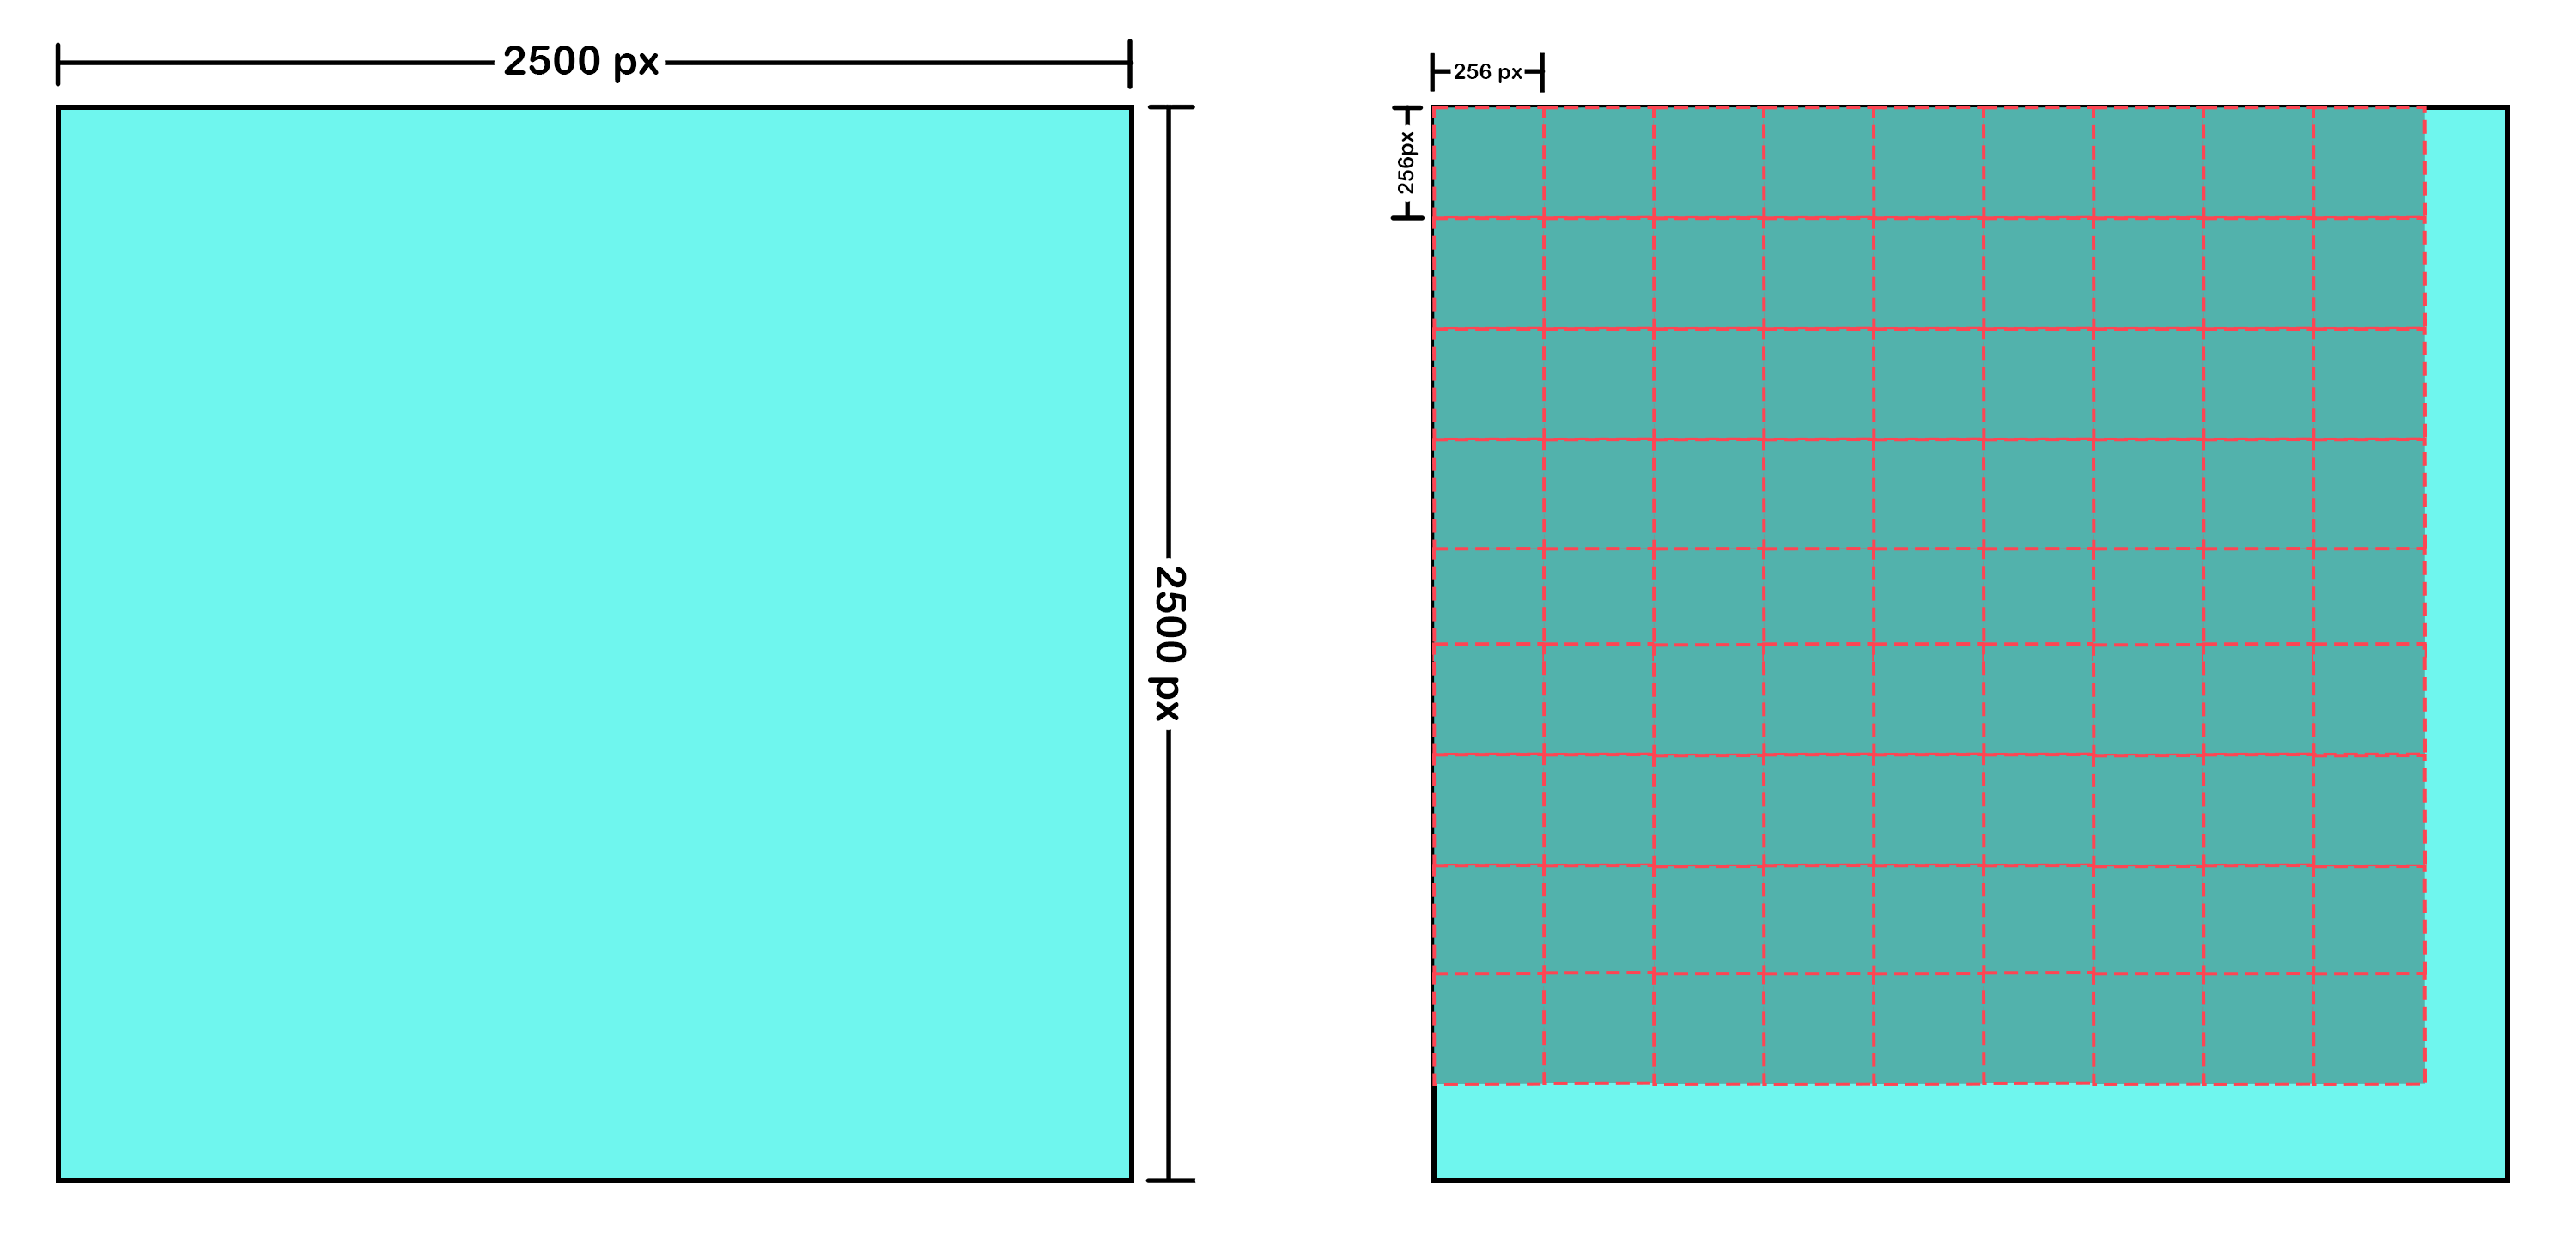
\includegraphics[width=\textwidth]{cropStep.png}
    \caption{Image demonstrating the step of cropping and dividing the large image into smaller images.}
    \label{fig:cropStep}
\end{figure*}

\subsubsection{Second manual inspection}
Once the images are cropped and divided into smaller images, one last manual inspection is performed. The purpose of this inspection is the same as the first manual inspection, to verify variations in images. This check is performed to ensure no plain images exist in the dataset.

\subsection{Google Earth Engine Method}
TODO for Ankana

\subsection{Augmenting Dataset with Heat Zone}
TODO for Shreyashi.

\subsection{Dataset availability}
To be filled later. Most probably dataset will be uploaded to kaggle and a doi will be generated for it.